%!TEX program = xelatex

% Name           : hsrm-beamer-minimal.sty
% Author         : Benjamin Weiss (benjamin.weiss@kreatiefton.de)
% Version        : 0.2
% Created on     : 08.05.2013
% Last Edited on : 24.03.2014
% Copyright      : Copyright (c) 2013 by Benjamin Weiss. All rights reserved.
% License        : This file may be distributed and/or modified under the
%                  GNU Public License.
% Description    : HSRM beamer theme minimal example.

\documentclass{beamer}

\usepackage[french]{babel}
\usepackage{datetime}

\usetheme[noflama]{hsrm}

\title{Rencontre AMOén}
\subtitle{Les derniers résultats des projets AMOén}
\author{Denis Iglesias}
%\institute{Studienbereich Informations- und Elektrotechnik\\Hochschule {\Medium RheinMain}}
\newdate{date}{04}{06}{2026}
\date{\displaydate{date}}

\begin{document}

\maketitle

\section*{Table des matières}
\begin{frame}{Table des matières}
	\tableofcontents[hideallsubsections]
\end{frame}

\section{Statut des projets}

\begin{frame}[t]{Statut des projets}
    \vspace{2pt}
    \collerGauche%
    \begin{minipage}[t]{0.38\paperwidth}
        \small
        \begin{itemize}
            \setlength{\itemsep}{0.4em}
            \item 80 projets
            \begin{itemize}
                \footnotesize
                \setlength{\itemsep}{0.3em}
                \item En cours ou finalisés
                \item 30 ancienne méthodologie
                \item 50 nouvelle méthodologie
                \item 4 projets sans bonus MI16
            \end{itemize}
            \item Terminés récemment
            \begin{itemize}
                \footnotesize
                \setlength{\itemsep}{0.3em}
                \item Adrien-Jeandin 4-6\_grange
                \item Dinu-Lipatti\_SPG
                \item Poste\_collex
                \item Vieusseux 16-18\_SCHG
            \end{itemize}
        \end{itemize}
    \end{minipage}%
    \begin{minipage}[t]{0.62\paperwidth}
        \vspace{0pt}
        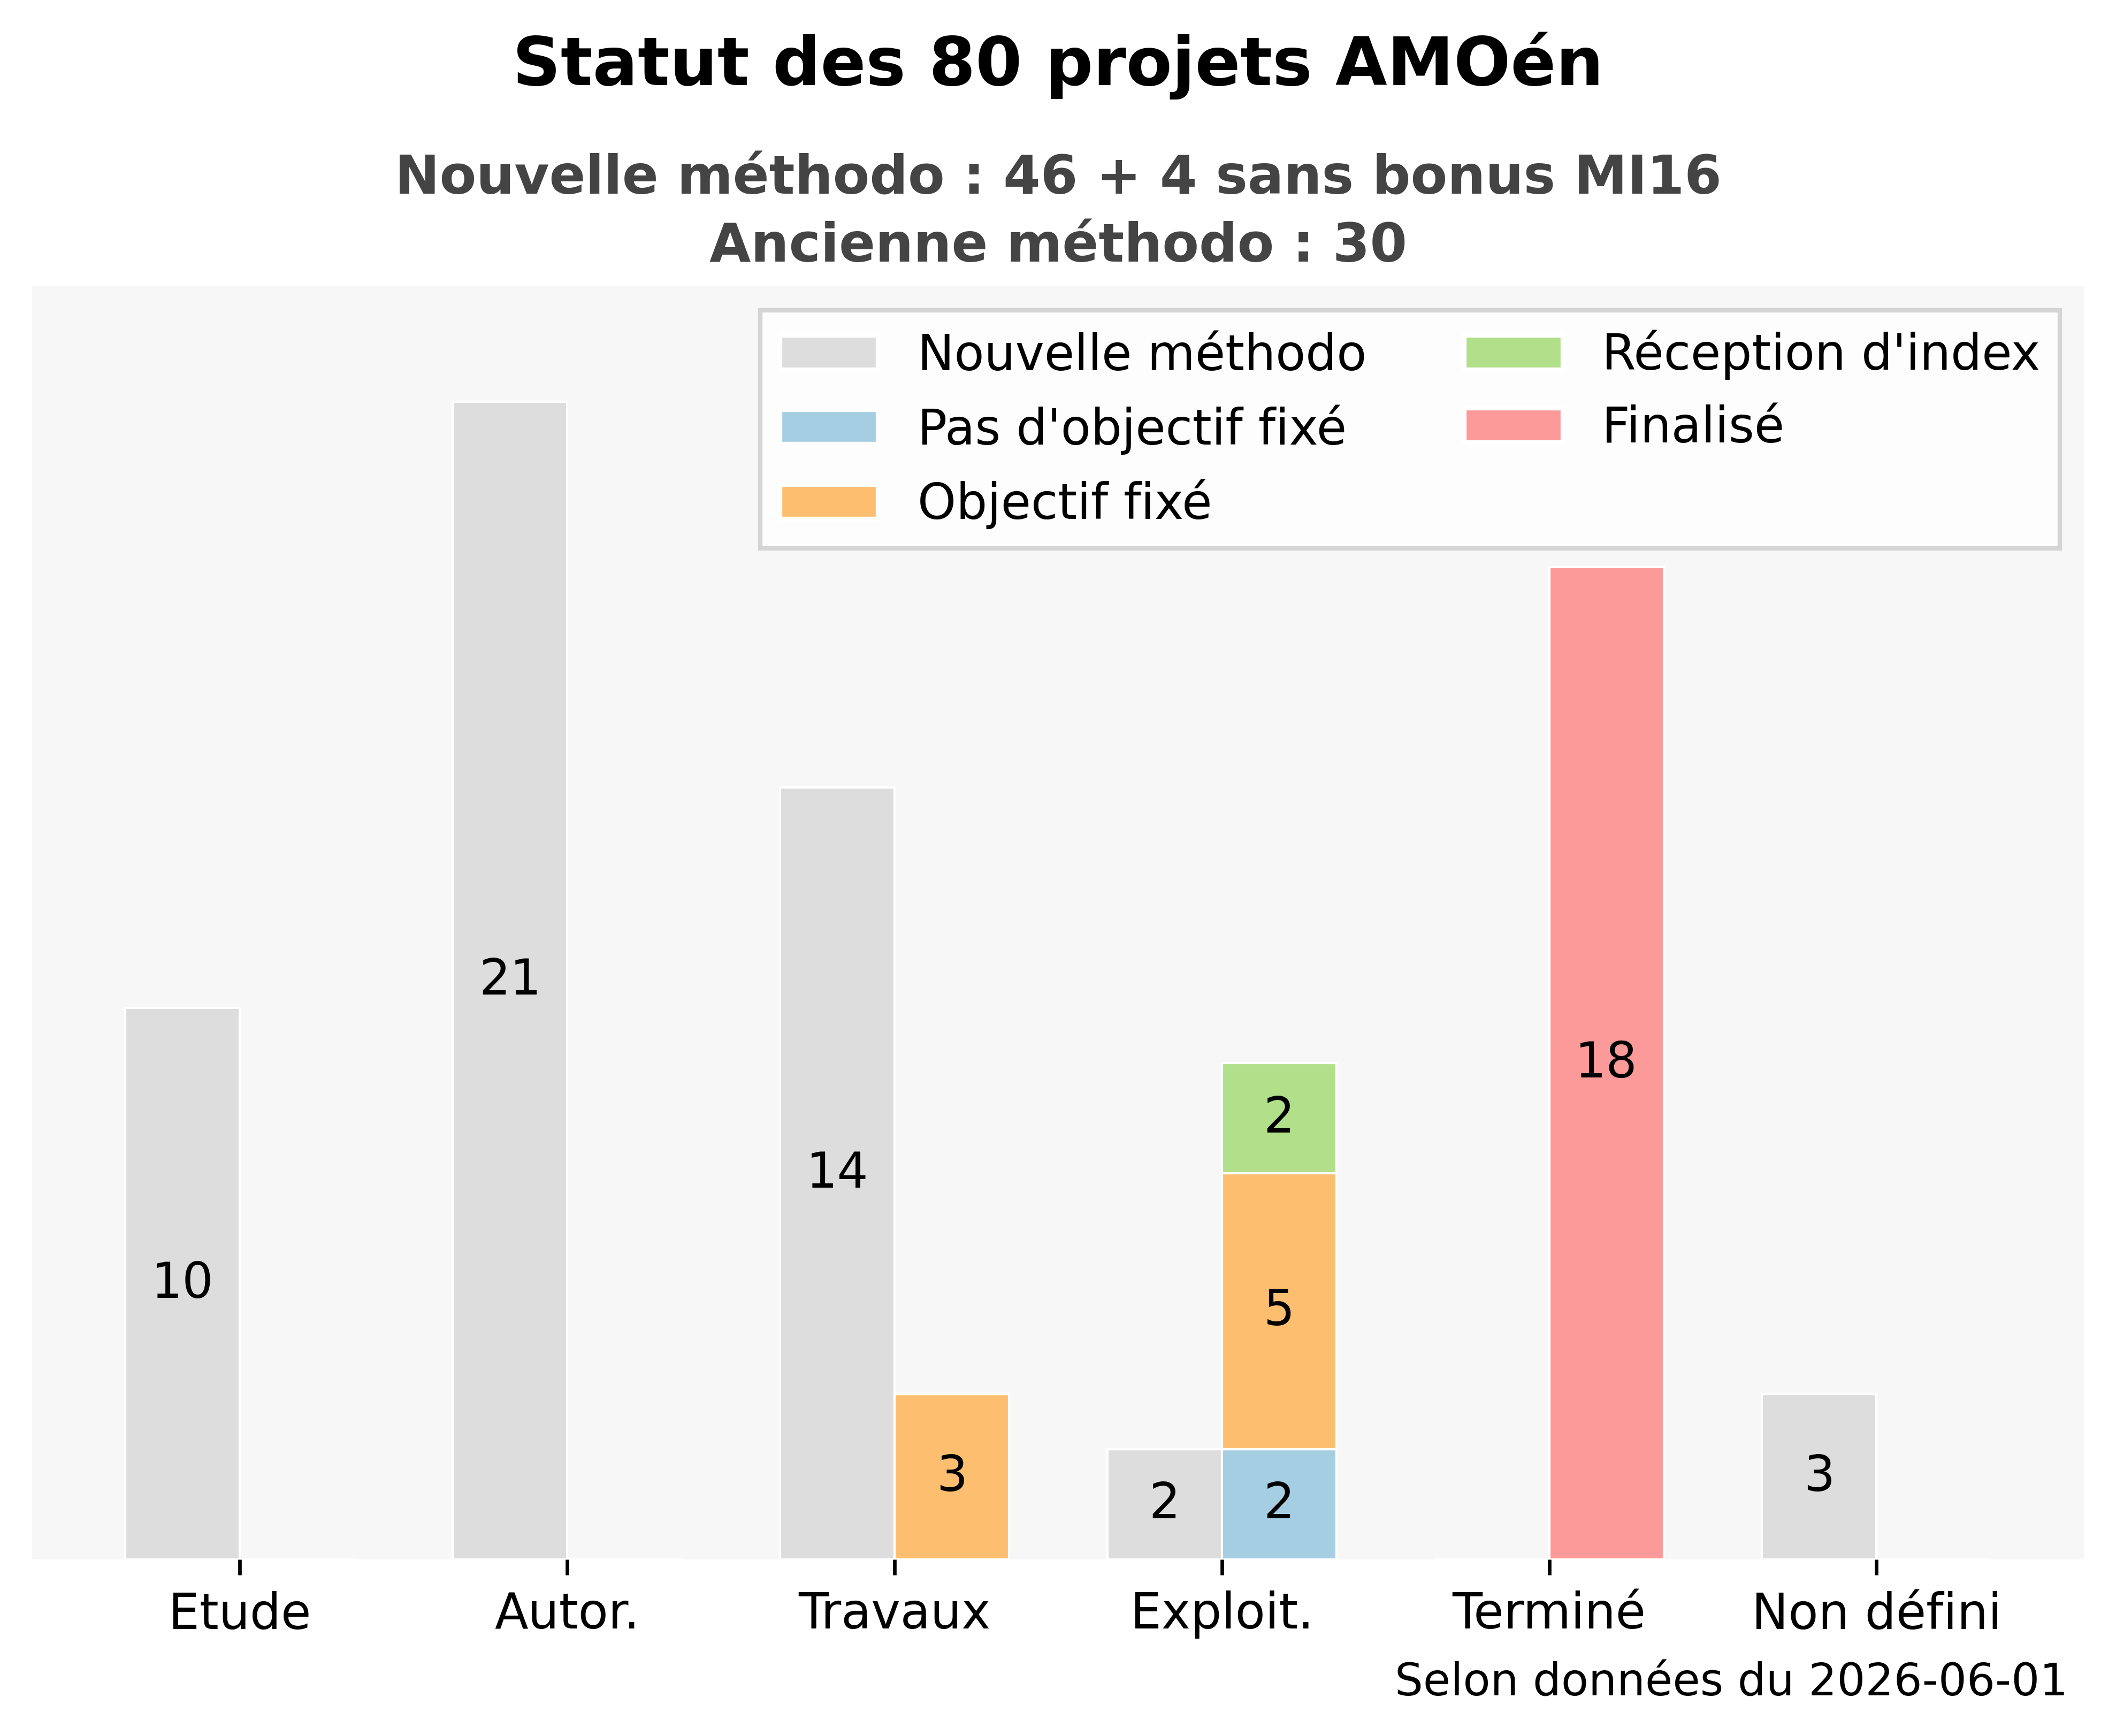
\includegraphics[
            width=\linewidth,
            height=0.80\textheight,
            keepaspectratio
        ]{img/01_statut_projets}
    \end{minipage}
\end{frame}

%---------------------------------------------------------------------
% performance
%---------------------------------------------------------------------

\section{Performance}

\begin{frame}[t]{Performance des sites en exploitation}
    \slideimage[0.69\textheight]{img/02_performance_sites_general_01_exploitation}%
	\vfill
	{\tiny Données indisponibles pour "Vernes-Vaudagne 16-18/41-45\_CPEG" et "Gilbert-Trolliet 2-12\_CAPetRealstone"}
\end{frame}

\begin{frame}[t]{Performance des sites récemment terminés}
    \slideimage[0.70\textheight]{img/02_performance_sites_general_02_termines_recent}
\end{frame}

% hauteur différente pour la dernière
\begin{frame}[t]{Performance des sites terminés}
    \slideimage[0.63\textheight]{img/02_performance_sites_general_03_termines}
    \vfill
    {\tiny "Michel-Chauvet 6-8" (projet pilote), "école Golette" et "Léchères 4\_Wincasa" (hors affectation logement collectif) ne sont pas inclus.}
\end{frame}

%---------------------------------------------------------------------
% performance vs IDC
%---------------------------------------------------------------------

\section{Comparatif IDC}

\begin{frame}[t]{Performance vs IDC 1/2}
    \slideimage[0.91\textheight]{img/02_performance_sites_general_04_termines_idc}
\end{frame}

\begin{frame}[t]{Performance vs IDC 2/2}
    \slideimage[0.91\textheight]{img/02_performance_sites_general_05_termines_idc}
\end{frame}

\begin{frame}[t]{Cas particulier 1/2: Avusy 10-10A}
    \vspace{2pt}

    % --- Image (top) ---
    {\centering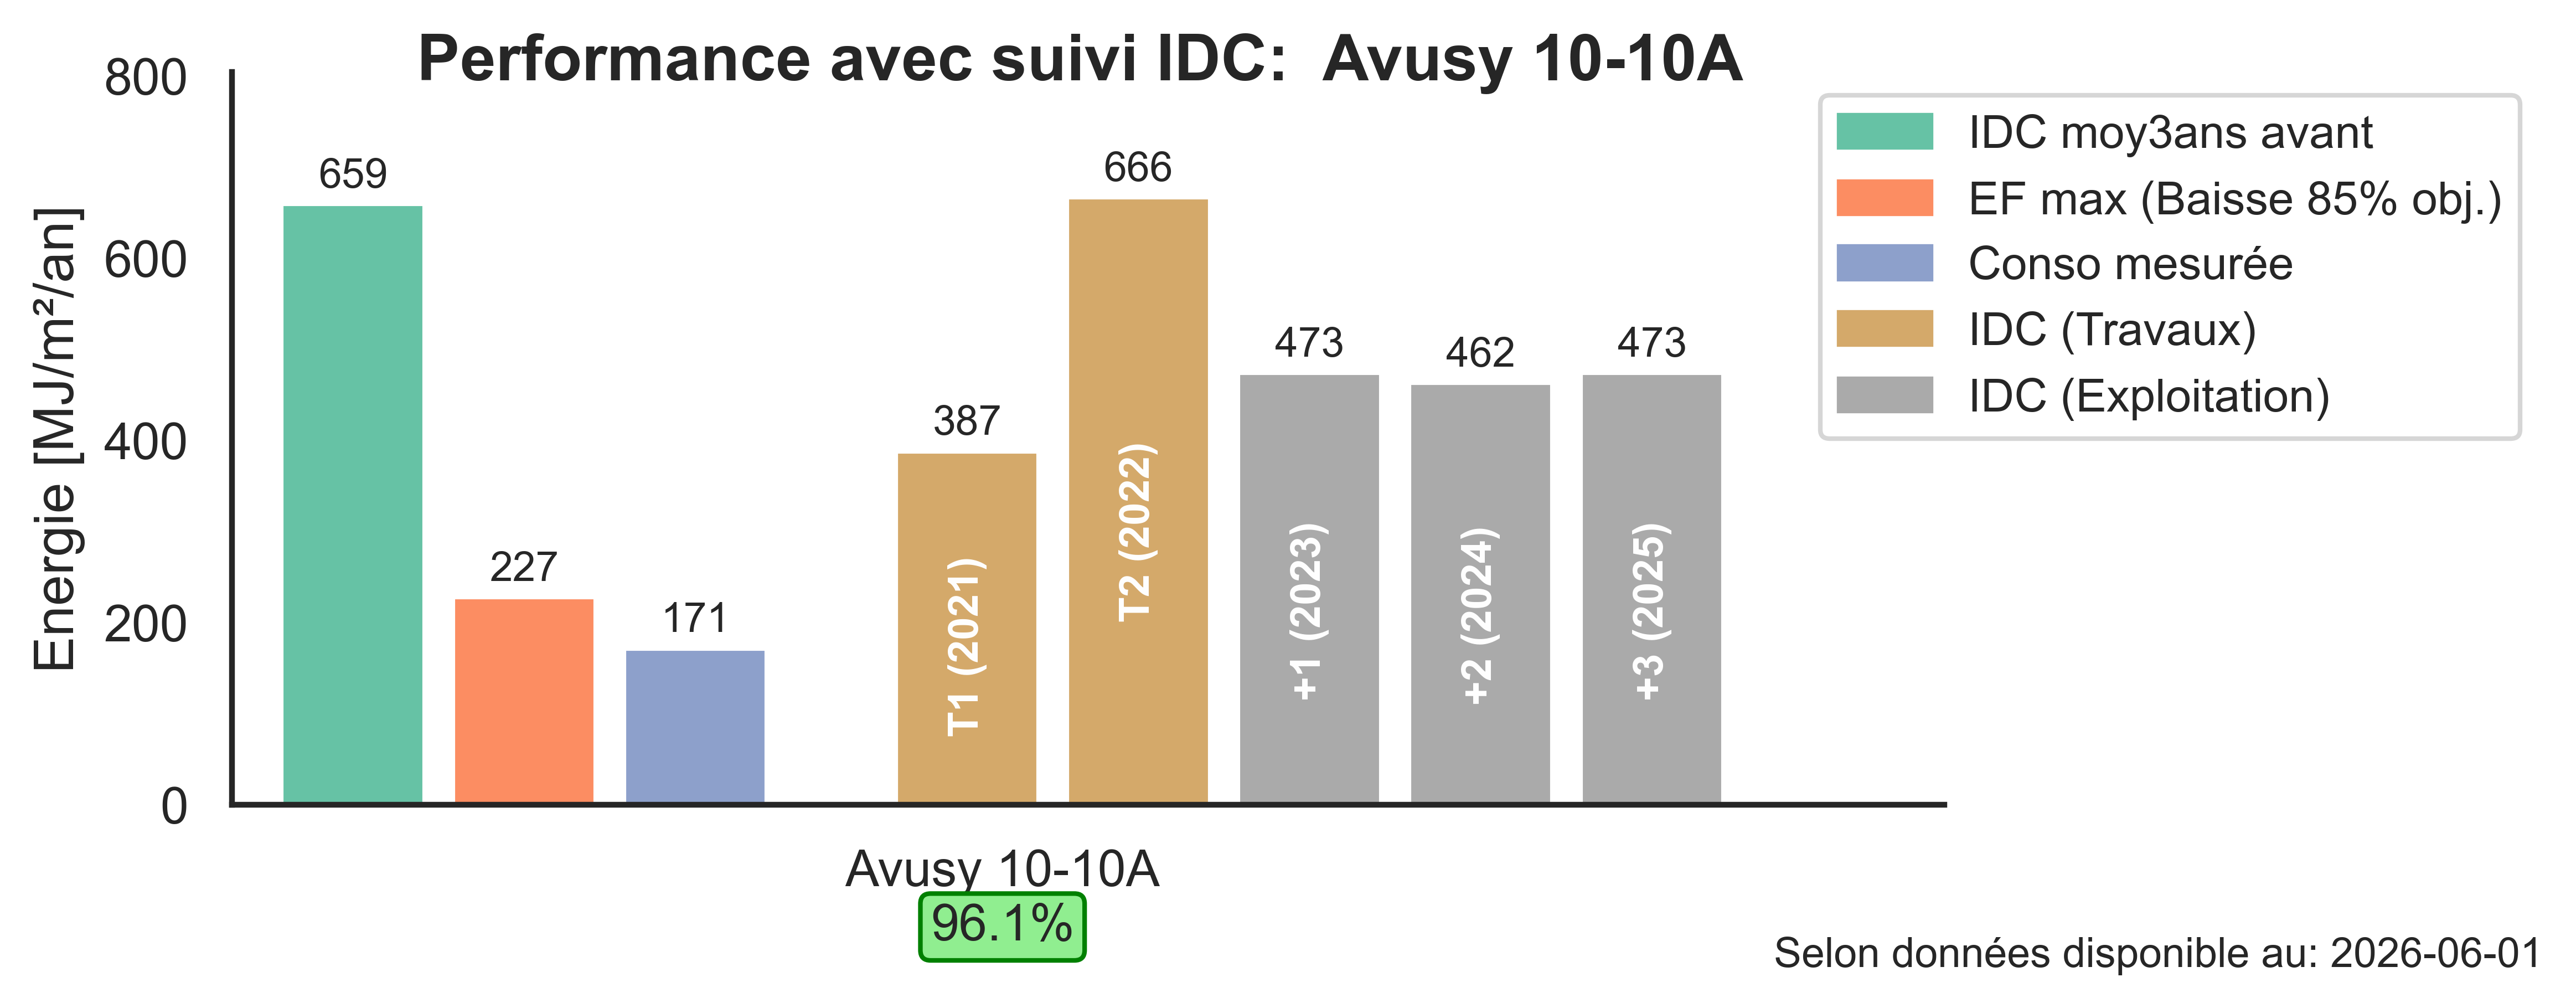
\includegraphics[
        width=\linewidth,
        height=0.42\textheight,
        keepaspectratio
    ]{img/02_performance_sites_general_06_cas_particulier_01}\par}

    \vfill

    % --- Table (bottom) ---
    {\footnotesize
    \begin{tabular}{lll}
        \hline
        \textbf{Paramètre} & \textbf{IDC}  & \textbf{AMOén} \\
        \hline
        SRE & 1620 m² & 1600 m²\\
        Consommation période (2025) & 187776 kWh (CAD) & 37104 kWh (élec PAC) \\
        \hline
    \end{tabular}}

    \vspace{8pt}
    {\small → Problème déclaration agent énergétique et quantité. Le bâtiment alimente aussi des villas à proximité, probablement que cette consommation n'a pas été retirée de l'immeuble (total 58969 kWh élec). Les villas n'ont pas été rénovées et consomment tout de même 37.1\% du total (21865 kWh).
    }

\end{frame}

\begin{frame}[t]{Cas particulier 2/2: Prulay 37-47}
    \vspace{2pt}

    % --- Image (top) ---
    {\centering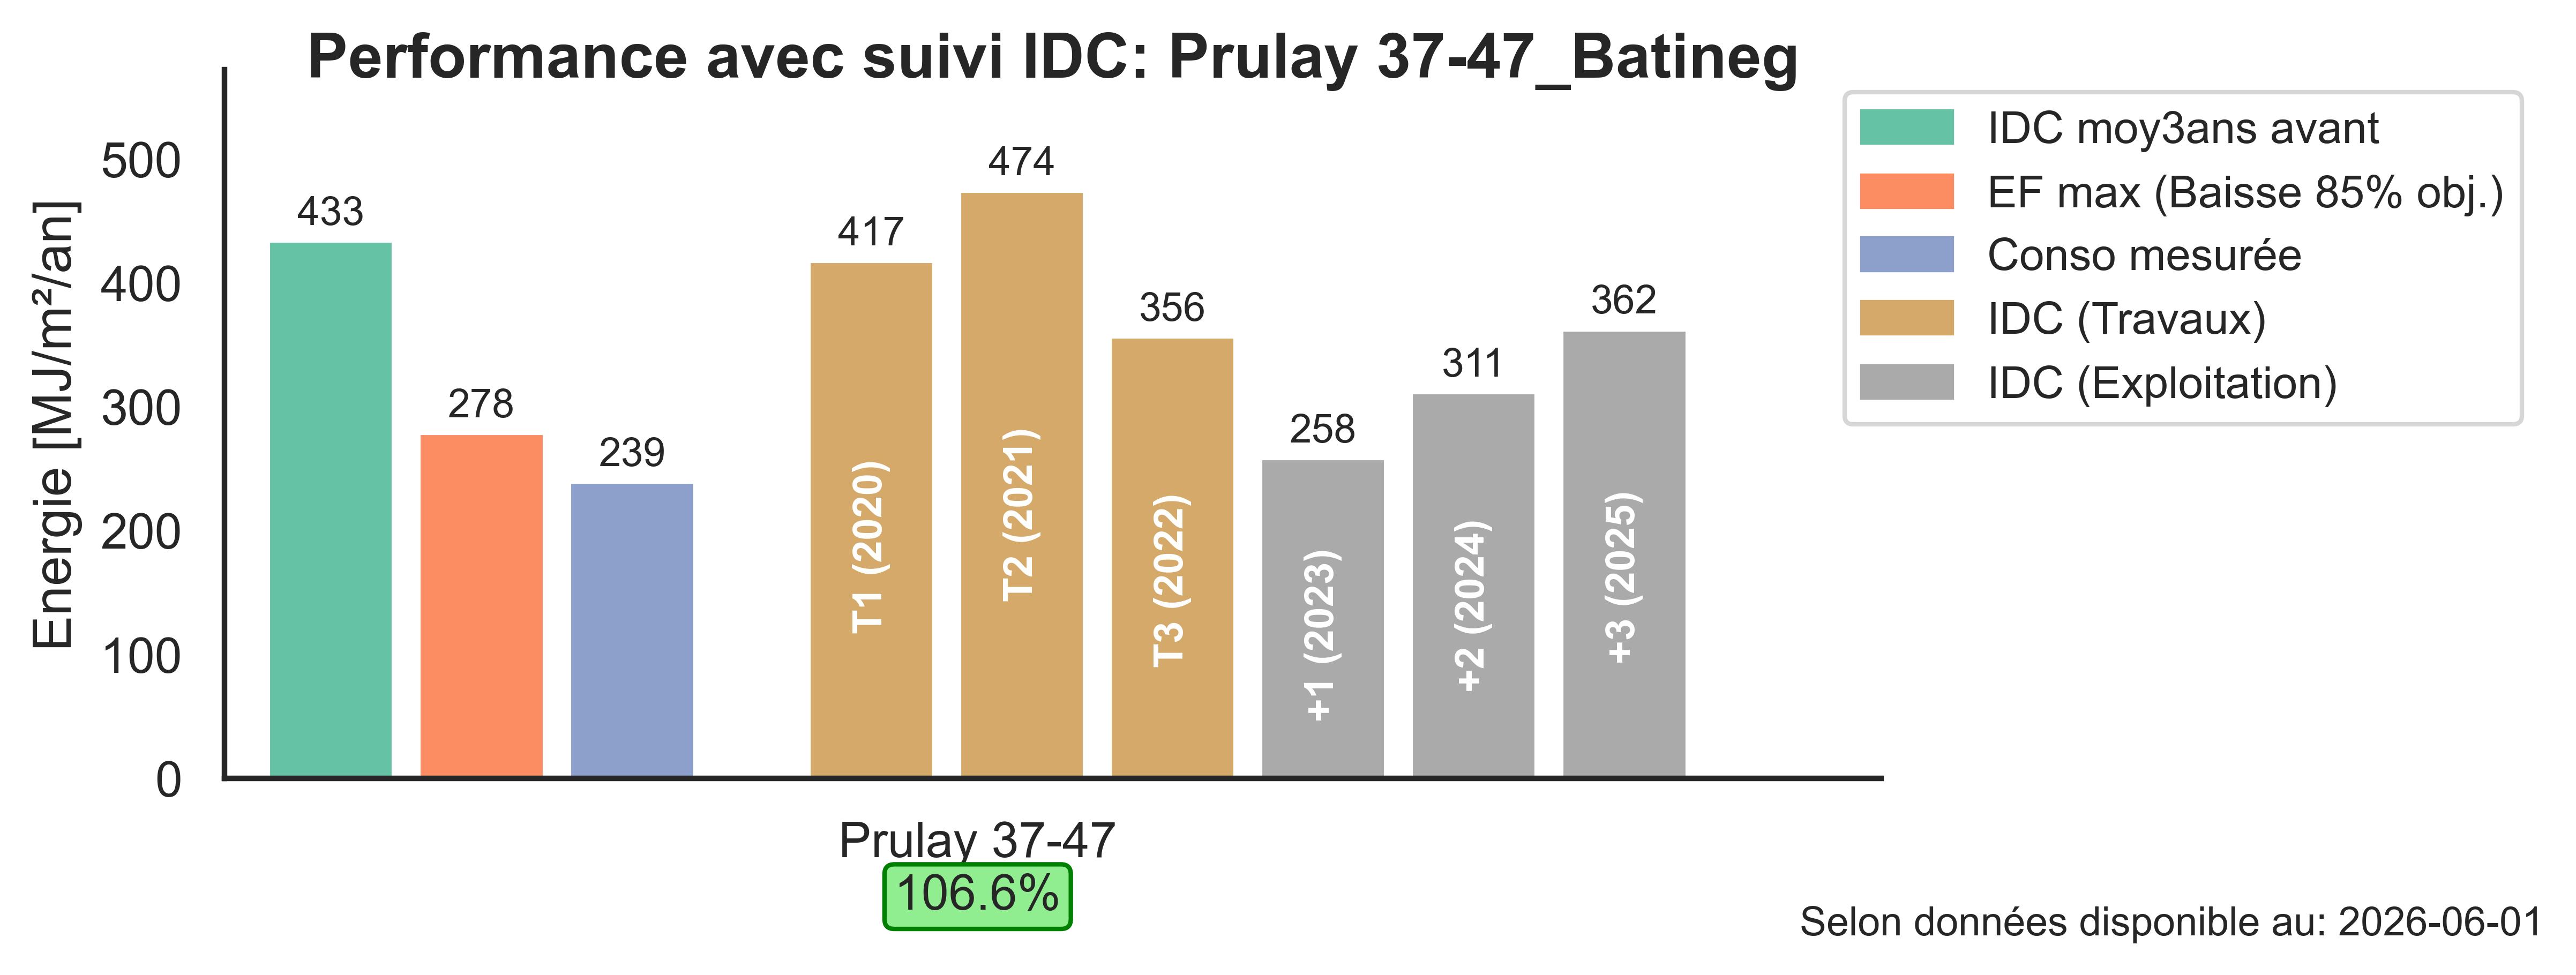
\includegraphics[
        width=\linewidth,
        height=0.42\textheight,
        keepaspectratio
    ]{img/02_performance_sites_general_06_cas_particulier_02}\par}

    \vfill

    {\small → L'augmentation de l'IDC observée à la fin du mandat AMOén indique une dégradation progressive des réglages fins réalisés en cours de suivi.}

\end{frame}

%---------------------------------------------------------------------
% Conclusion
%---------------------------------------------------------------------

\section{Conclusion}
\begin{frame}[t]{Conclusion}
    \vspace{4pt}
    \begin{itemize}
        \setlength{\itemsep}{0.5em}
        \item 80 sites dont 30 selon ancienne méthodologie :
        \begin{itemize}
            \setlength{\itemsep}{0.2em}
            \item 3 en travaux
            \item 9 en exploitation
            \item 18 terminés
        \end{itemize}
        \item Performance atteinte dans 13 cas sur 14
        \item Comparatif IDC :
        \begin{itemize}
            \setlength{\itemsep}{0.2em}
            \item Tendance IDC à la baisse après rénovation
            \item Calcul PAC COP: IDC (3.25) vs AMOén (2.5)
            \item 2 cas particuliers analysés
        \end{itemize}
    \end{itemize}
\end{frame}

\end{document}






